\section{Relic density constraints for $b-$flavored Dark Matter}
\label{app:Relic_Density_bFDM}

For Dirac fermion DM the relic density is governed primarily by the $s$-wave annihilation cross section, which is given approximately given by:
\begin{equation}
\langle \sigma v \rangle = \frac{3g^4}{32\pi} \frac{m^2_\chi \sqrt{1-(m_b/m_\chi)^2}}{\left( m^2_\Phi+m^2_\chi-m^2_b \right)} \approx \frac{3g^4 m^2_\chi}{32\pi (m^2_\Phi+m^2_\chi)}
\end{equation}

We assume $ \langle \sigma v \rangle=1.5$~pb. 

%For Majorana fermion DM the relic density is governed primarily by the $p$-wave annihilation cross section, which is given approximately by
%\begin{equation}
% \langle \sigma v \rangle \approx a+bv^2,~ b=g^4\frac{m^2_\chi (m^4_B + m^4_\chi)}{16 \pi (m^2_B+m^2_\chi)}
%\end{equation}

Figure~\ref{fig:relic_weights} shows the weights obtained for various dark matter and mediator massed required to obtain the correct relic density observed in the early universe.

\begin{figure}[h!]
	\centering 
	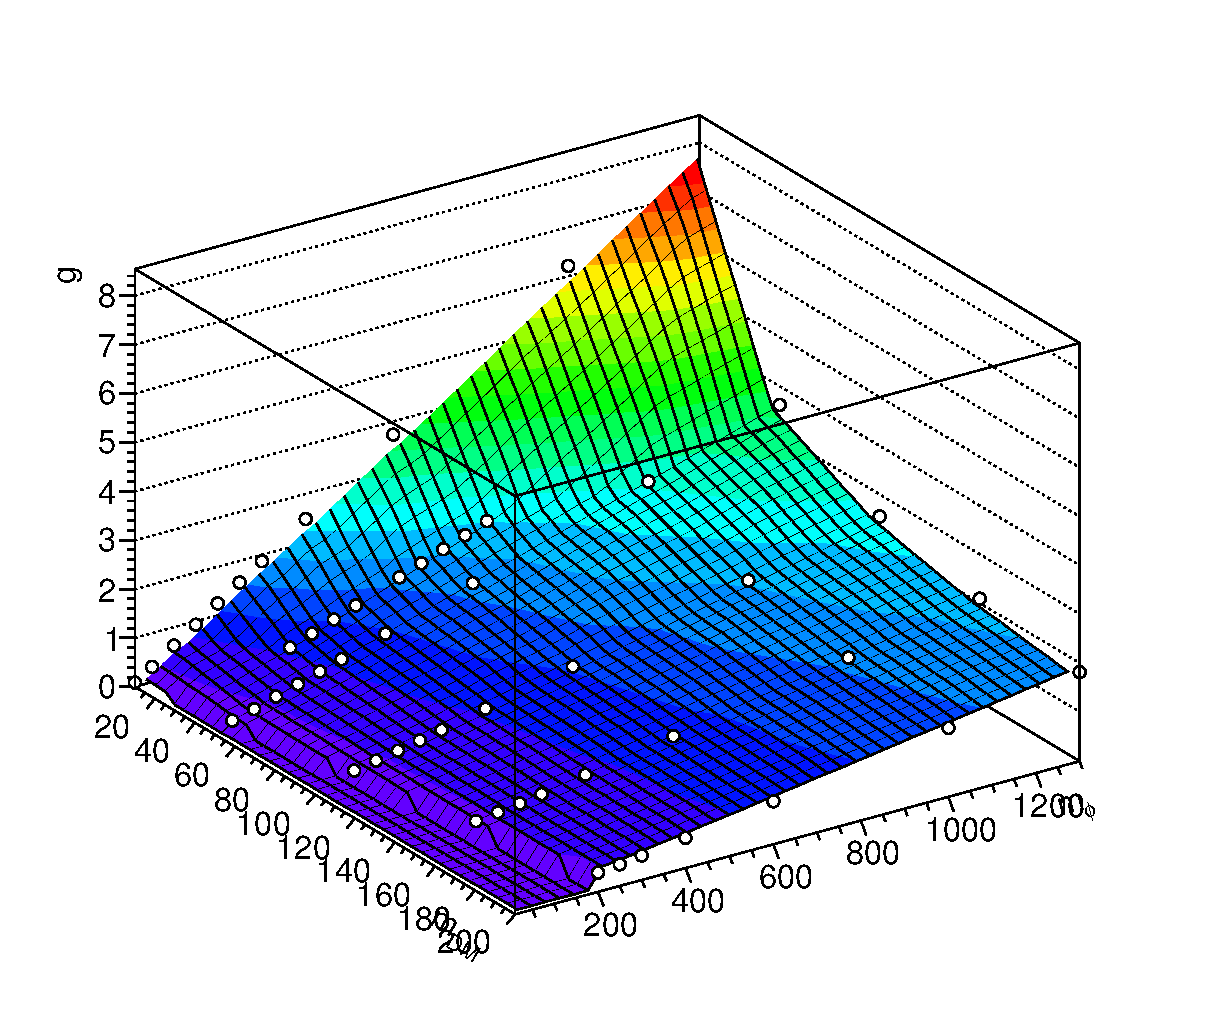
\includegraphics[scale=0.5]{figures/bFDM/relic_weights.eps}
	\caption{Coupling constants required to obtain correct relic density in the early universe . \label{fig:relic_weights}}
	\end{figure}	
	
\section{Cross sections for $b-$flavored Dark Matter}
\label{app:xsecs_bFDM}

\begin{table}[h]
	\centering
	\begin{tabular}{lll|lll}
		\hline \hline
		$m_\chi $  & $m_\Phi$ & $\sigma$ [pb] & $m_\chi $  & $m_\Phi$ & $\sigma$ [pb]\\ \hline \hline
		100 & 1000 & 5.48E-03 & 150 & 600  & 1.23E-01 \\\hline
		100 & 100  & 1.91E-02 & 200 & 1000 & 4.94E-03 \\\hline
		100 & 1300 & 8.90E-04 & 200 & 1300 & 7.82E-04 \\\hline
		100 & 150  & 6.66E+00 & 200 & 200  & 2.66E-03 \\\hline
		100 & 200  & 9.86E+00 & 200 & 250  & 6.48E-01 \\\hline
		100 & 250  & 7.67E+00 & 200 & 300  & 1.69E+00 \\\hline
		100 & 300  & 4.12E+00 & 200 & 400  & 9.41E-01 \\\hline
		100 & 400  & 1.11E+00 & 200 & 600  & 1.16E-01 \\\hline
		100 & 600  & 1.30E-01 & 35  & 250  & 9.75E+00 \\\hline
		10  & 1000 & 5.80E-03 & 35  & 300  & 4.56E+00 \\\hline
		10  & 100  & 7.84E+01 & 35  & 350  & 2.22E+00 \\\hline
		10  & 10   & 4.09E-01 & 35  & 400  & 1.19E+00 \\\hline
		10  & 1300 & 9.53E-04 & 35  & 500  & 3.76E-01 \\\hline
		10  & 150  & 3.95E+01 & 35  & 550  & 2.24E-01 \\\hline
		10  & 200  & 2.12E+01 & 35  & 600  & 1.37E-01 \\\hline
		10  & 250  & 9.92E+00 & 35  & 650  & 8.62E-02 \\\hline
		10  & 300  & 4.57E+00 & 35  & 700  & 5.54E-02 \\\hline
		10  & 400  & 1.20E+00 & 50  & 1000 & 5.72E-03 \\\hline
		10  & 50   & 1.59E+02 & 50  & 100  & 3.25E+01 \\\hline
		10  & 600  & 1.38E-01 & 50  & 1300 & 9.34E-04 \\\hline
		150 & 1000 & 5.22E-03 & 50  & 150  & 2.84E+01 \\\hline
		150 & 1300 & 8.37E-04 & 50  & 200  & 1.84E+01 \\\hline
		150 & 150  & 6.64E-03 & 50  & 250  & 9.52E+00 \\\hline
		150 & 200  & 1.87E+00 & 50  & 300  & 4.49E+00 \\\hline
		150 & 250  & 3.86E+00 & 50  & 400  & 1.17E+00 \\\hline
		150 & 300  & 3.35E+00 & 50  & 50   & 7.06E-02 \\\hline
		150 & 400  & 1.03E+00 & 50  & 600  & 1.36E-01 \\\hline
		\hline
	\end{tabular}
	\caption{Dark matter masses $m_{\chi}$ and mediator masses $m_{\Phi}$ generated for $g=1$ for 13 TeV. The resulting
		production cross sections are given in pb.\label{tab:g1_13T}}
\end{table}


\begin{table}[h]
	\centering
	\begin{tabular}{lll|lll}
		\hline \hline
		$m_\chi $  & $m_\Phi$ & $\sigma$ [pb] & $m_\chi $  & $m_\Phi$ & $\sigma$ [pb]\\ \hline \hline
		100 & 1000 & 1.50E-02 & 150 & 600  & 1.22E-01 \\\hline
		100 & 100  & 1.13E-04 & 200 & 1000 & 7.04E-03 \\\hline
		100 & 1300 & 7.05E-03 & 200 & 1300 & 2.11E-03 \\\hline
		100 & 150  & 6.12E+00 & 200 & 200  & 6.29E-05 \\\hline
		100 & 200  & 9.60E+00 & 200 & 250  & 5.83E-01 \\\hline
		100 & 250  & 7.57E+00 & 200 & 300  & 1.64E+00 \\\hline
		100 & 300  & 4.01E+00 & 200 & 400  & 9.08E-01 \\\hline
		100 & 400  & 1.06E+00 & 200 & 600  & 1.11E-01 \\\hline
		100 & 600  & 1.45E-01 & 35  & 250  & 9.62E+00 \\\hline
		10  & 1000 & 3.55E-01 & 35  & 300  & 4.56E+00 \\\hline
		10  & 100  & 7.67E+01 & 35  & 350  & 2.35E+00 \\\hline
		10  & 10   & 2.43E-05 & 35  & 400  & 1.33E+00 \\\hline
		10  & 1300 & 2.35E-01 & 35  & 500  & 5.48E-01 \\\hline
		10  & 150  & 3.92E+01 & 35  & 550  & 3.80E-01 \\\hline
		10  & 200  & 2.13E+01 & 35  & 600  & 2.76E-01 \\\hline
		10  & 250  & 1.05E+01 & 35  & 650  & 2.07E-01 \\\hline
		10  & 300  & 5.57E+00 & 35  & 700  & 1.60E-01 \\\hline
		10  & 400  & 2.35E+00 & 50  & 1000 & 3.69E-02 \\\hline
		10  & 50   & 1.51E+02 & 50  & 100  & 3.07E+01 \\\hline
		10  & 600  & 8.16E-01 & 50  & 1300 & 2.39E-02 \\\hline
		150 & 1000 & 9.44E-03 & 50  & 150  & 2.76E+01 \\\hline
		150 & 1300 & 3.44E-03 & 50  & 200  & 1.82E+01 \\\hline
		150 & 150  & 8.84E-05 & 50  & 250  & 9.31E+00 \\\hline
		150 & 200  & 1.69E+00 & 50  & 300  & 4.40E+00 \\\hline
		150 & 250  & 3.76E+00 & 50  & 400  & 1.22E+00 \\\hline
		150 & 300  & 3.29E+00 & 50  & 50   & 1.04E-04 \\\hline
		150 & 400  & 9.83E-01 & 50  & 600  & 2.14E-01 \\\hline
		\hline
	\end{tabular}
	\caption{Dark matter masses $m_{\chi}$ and mediator masses $m_{\Phi}$ generated such that relic density constraints are fullfilled for 13 TeV. The resulting
		production cross sections are given in pb.\label{tab:g_relic_13T}}
\end{table}

\begin{table}[h]
	\centering
	\begin{tabular}{lll|lll}
		\hline \hline
		$m_\chi $  & $m_\Phi$ & $\sigma$ [pb] & $m_\chi $  & $m_\Phi$ & $\sigma$ [pb]\\ \hline \hline
		100 & 1000 & 1.50E-02 & 150 & 600  & 1.22E-01 \\\hline
		100 & 100  & 1.13E-04 & 200 & 1000 & 7.04E-03 \\\hline
		100 & 1300 & 7.05E-03 & 200 & 1300 & 2.11E-03 \\\hline
		100 & 150  & 6.12E+00 & 200 & 200  & 6.29E-05 \\\hline
		100 & 200  & 9.60E+00 & 200 & 250  & 5.83E-01 \\\hline
		100 & 250  & 7.57E+00 & 200 & 300  & 1.64E+00 \\\hline
		100 & 300  & 4.01E+00 & 200 & 400  & 9.08E-01 \\\hline
		100 & 400  & 1.06E+00 & 200 & 600  & 1.11E-01 \\\hline
		100 & 600  & 1.45E-01 & 35  & 250  & 9.62E+00 \\\hline
		10  & 1000 & 3.55E-01 & 35  & 300  & 4.56E+00 \\\hline
		10  & 100  & 7.67E+01 & 35  & 350  & 2.35E+00 \\\hline
		10  & 10   & 2.43E-05 & 35  & 400  & 1.33E+00 \\\hline
		10  & 1300 & 2.35E-01 & 35  & 500  & 5.48E-01 \\\hline
		10  & 150  & 3.92E+01 & 35  & 550  & 3.80E-01 \\\hline
		10  & 200  & 2.13E+01 & 35  & 600  & 2.76E-01 \\\hline
		10  & 250  & 1.05E+01 & 35  & 650  & 2.07E-01 \\\hline
		10  & 300  & 5.57E+00 & 35  & 700  & 1.60E-01 \\\hline
		10  & 400  & 2.35E+00 & 50  & 1000 & 3.69E-02 \\\hline
		10  & 50   & 1.51E+02 & 50  & 100  & 3.07E+01 \\\hline
		10  & 600  & 8.16E-01 & 50  & 1300 & 2.39E-02 \\\hline
		150 & 1000 & 9.44E-03 & 50  & 150  & 2.76E+01 \\\hline
		150 & 1300 & 3.44E-03 & 50  & 200  & 1.82E+01 \\\hline
		150 & 150  & 8.84E-05 & 50  & 250  & 9.31E+00 \\\hline
		150 & 200  & 1.69E+00 & 50  & 300  & 4.40E+00 \\\hline
		150 & 250  & 3.76E+00 & 50  & 400  & 1.22E+00 \\\hline
		150 & 300  & 3.29E+00 & 50  & 50   & 1.04E-04 \\\hline
		150 & 400  & 9.83E-01 & 50  & 600  & 2.14E-01 \\\hline
		\hline
	\end{tabular}
	\caption{Dark matter masses $m_{\chi}$ and mediator masses $m_{\Phi}$ generated such that relic density constraints are fullfilled for 13 TeV. The resulting
		production cross sections are given in pb.\label{tab:g_relic_13T}}
\end{table}


\begin{table}[h]
	\centering
	\begin{tabular}{lll|lll}
		\hline \hline
		$m_\chi $  & $m_\Phi$ & $\sigma$ [pb] & $m_\chi $  & $m_\Phi$ & $\sigma$ [pb]\\ \hline \hline
		100 & 1000 & 1.53E-03 & 150 & 600  & 1.61E-02 \\\hline
		100 & 100  & 2.21E-05 & 200 & 1000 & 5.46E-04 \\\hline
		100 & 1300 & 7.91E-04 & 200 & 1300 & 1.54E-04 \\\hline
		100 & 150  & 1.58E+00 & 200 & 200  & 9.52E-06 \\\hline
		100 & 200  & 2.48E+00 & 200 & 250  & 1.22E-01 \\\hline
		100 & 250  & 1.82E+00 & 200 & 300  & 3.53E-01 \\\hline
		100 & 300  & 8.77E-01 & 200 & 400  & 1.65E-01 \\\hline
		100 & 400  & 1.94E-01 & 200 & 600  & 1.43E-02 \\\hline
		100 & 600  & 2.00E-02 & 35  & 250  & 2.32E+00 \\\hline
		10  & 1000 & 5.61E-02 & 35  & 300  & 1.00E+00 \\\hline
		10  & 100  & 2.36E+01 & 35  & 350  & 4.73E-01 \\\hline
		10  & 10   & 6.53E-06 & 35  & 400  & 2.51E-01 \\\hline
		10  & 1300 & 3.62E-02 & 35  & 500  & 9.23E-02 \\\hline
		10  & 150  & 1.12E+01 & 35  & 550  & 6.07E-02 \\\hline
		10  & 200  & 5.61E+00 & 35  & 600  & 4.20E-02 \\\hline
		10  & 250  & 2.50E+00 & 35  & 650  & 3.02E-02 \\\hline
		10  & 300  & 1.21E+00 & 35  & 700  & 2.25E-02 \\\hline
		10  & 400  & 4.53E-01 & 50  & 1000 & 4.70E-03 \\\hline
		10  & 50   & 4.83E+01 & 50  & 100  & 8.88E+00 \\\hline
		10  & 600  & 1.34E-01 & 50  & 1300 & 3.34E-03 \\\hline
		150 & 1000 & 8.21E-04 & 50  & 150  & 7.83E+00 \\\hline
		150 & 1300 & 3.07E-04 & 50  & 200  & 4.80E+00 \\\hline
		150 & 150  & 1.52E-05 & 50  & 250  & 2.25E+00 \\\hline
		150 & 200  & 3.93E-01 & 50  & 300  & 9.67E-01 \\\hline
		150 & 250  & 8.86E-01 & 50  & 400  & 2.28E-01 \\\hline
		150 & 300  & 7.19E-01 & 50  & 50   & 2.37E-05 \\\hline
		150 & 400  & 1.79E-01 & 50  & 600  & 3.15E-02 \\\hline
		\hline
	\end{tabular}
	\caption{Dark matter masses $m_{\chi}$ and mediator masses $m_{\Phi}$ generated for such that relic density constraints are fullfilled for 8 TeV. The resulting
		production cross sections are given in pb.\label{tab:g_relic_8T}}
\end{table}



\section{Cross sections for the $t\bar t$+DM scalar simplified model}

\begin{longtable}{lllll}
	\caption{Cross section calculation for each coupling choice and minimal width assumption for the $t\bar t$+DM scalar simplified model grid}\\
	\toprule
	Coupling (g) & $m_{Phi}$ [GeV] & $m_{\chi}$ [GeV] & $\Gamma_{min}$ [GeV] & $\sigma$ [pb]\\
	\midrule
	\endfirsthead
	
	\multicolumn{5}{c}{\tablename\ \thetable{} -- continued from previous page} \\
	Coupling (g) & $m_{Phi}$ [GeV] & $m_{\chi}$ [GeV] & $\Gamma_{min}$ [GeV] & $\sigma$ [pb]\\
	\midrule
	\endhead
	
	\midrule
	\multicolumn{5}{r}{{Continued on next page}} \\ 
	\endfoot
	
	\bottomrule
	\endlastfoot
	0.1 & 10 & 1 & 0.00374 & 0.1955 $\pm$ 0.00066 \\
	0.1 & 20 & 1 & 0.00785 & 0.1054 $\pm$ 0.00031 \\
	0.1 & 50 & 1 & 0.0199 & 0.03011 $\pm$ 9.1e-05 \\
	0.1 & 100 & 1 & 0.0398 & 0.006867 $\pm$ 2.5e-05 \\
	0.1 & 200 & 1 & 0.0797 & 0.0009397 $\pm$ 2.6e-06 \\
	0.1 & 300 & 1 & 0.120 & 0.0002942 $\pm$ 1e-06 \\
	0.1 & 500 & 1 & 0.311 & 5.289e-05 $\pm$ 1.9e-07 \\
	0.1 & 1000 & 1 & 0.881 & 3.717e-06 $\pm$ 1.5e-08 \\
	0.1 & 2000 & 1 & 1.91 & 7.81e-08 $\pm$ 3.2e-10 \\
	0.1 & 5000 & 1 & 4.89 & 1.111e-11 $\pm$ 5.5e-14 \\
	0.1 & 10 & 10 & 6.33 & 9.418e-06 $\pm$ 3.6e-08 \\
	0.1 & 50 & 10 & 0.0153 & 0.03016 $\pm$ 8.1e-05 \\
	0.1 & 100 & 10 & 0.0375 & 0.00686 $\pm$ 2.2e-05 \\
	0.1 & 5000 & 10 & 4.89 & 1.095e-11 $\pm$ 5.8e-14 \\
	0.1 & 15 & 10 & 3.84 & 1.2e-05 $\pm$ 4.8e-08 \\
	0.1 & 10 & 50 & 6.33 & 1.914e-07 $\pm$ 7.2e-10 \\
	0.1 & 50 & 50 & 2.34e-05 & 2.323e-07 $\pm$ 8.8e-10 \\
	0.1 & 200 & 50 & 0.0518 & 0.0009421 $\pm$ 2.8e-06 \\
	0.1 & 300 & 50 & 0.100 & 0.0002954 $\pm$ 9.8e-07 \\
	0.1 & 5000 & 50 & 4.88 & 1.059e-11 $\pm$ 5.3e-14 \\
	0.1 & 95 & 50 & 4.66e-05 & 6.548e-07 $\pm$ 2.3e-09 \\
	0.1 & 10 & 150 & 6.33 & 8.684e-09 $\pm$ 4.1e-11 \\
	0.1 & 200 & 150 & 0.000107 & 1.296e-08 $\pm$ 5.3e-11 \\
	0.1 & 500 & 150 & 0.214 & 3.92e-05 $\pm$ 1.6e-07 \\
	0.1 & 5000 & 150 & 4.87 & 9.079e-12 $\pm$ 5.9e-14 \\
	0.1 & 295 & 150 & 0.000185 & 3.969e-08 $\pm$ 2e-10 \\
	0.1 & 10 & 500 & 6.33 & 7.367e-11 $\pm$ 3.2e-13 \\
	0.1 & 500 & 500 & 0.112 & 9.86e-11 $\pm$ 3.9e-13 \\
	0.1 & 2000 & 500 & 1.63 & 5.953e-08 $\pm$ 2.3e-10 \\
	0.1 & 5000 & 500 & 4.77 & 5.768e-12 $\pm$ 2.6e-14 \\
	0.1 & 995 & 500 & 0.480 & 8.67e-10 $\pm$ 3.6e-12 \\
	0.1 & 10 & 1000 & 6.33 & 6.576e-13 $\pm$ 2.8e-15 \\
	0.1 & 1000 & 1000 & 0.483 & 9.426e-13 $\pm$ 4.2e-15 \\
	0.1 & 5000 & 1000 & 4.43 & 4.314e-12 $\pm$ 2e-14 \\
	0.1 & 1995 & 1000 & 1.11 & 1.589e-11 $\pm$ 9.2e-14 \\
	0.3 & 10 & 1 & 0.0337 & 1.766 $\pm$ 0.006 \\
	0.3 & 20 & 1 & 0.0706 & 0.9493 $\pm$ 0.0029 \\
	0.3 & 50 & 1 & 0.179 & 0.2695 $\pm$ 0.00082 \\
	0.3 & 100 & 1 & 0.358 & 0.06159 $\pm$ 0.00021 \\
	0.3 & 200 & 1 & 0.717 & 0.008466 $\pm$ 2.4e-05 \\
	0.3 & 300 & 1 & 1.08 & 0.002649 $\pm$ 8.5e-06 \\
	0.3 & 500 & 1 & 2.80 & 0.0004741 $\pm$ 1.6e-06 \\
	0.3 & 1000 & 1 & 7.93 & 3.349e-05 $\pm$ 1.3e-07 \\
	0.3 & 2000 & 1 & 17.2 & 7.227e-07 $\pm$ 3.2e-09 \\
	0.3 & 5000 & 1 & 44.0 & 5.42e-10 $\pm$ 3.5e-12 \\
	0.3 & 10 & 10 & 5.70 & 0.0007633 $\pm$ 2.5e-06 \\
	0.3 & 50 & 10 & 0.138 & 0.2706 $\pm$ 0.00082 \\
	0.3 & 100 & 10 & 0.337 & 0.06182 $\pm$ 0.00022 \\
	0.3 & 5000 & 10 & 44.0 & 5.386e-10 $\pm$ 2.7e-12 \\
	0.3 & 15 & 10 & 3.45e-05 & 0.0009761 $\pm$ 3.6e-06 \\
	0.3 & 10 & 50 & 5.70 & 1.561e-05 $\pm$ 6.1e-08 \\
	0.3 & 50 & 50 & 0.000210 & 1.892e-05 $\pm$ 7.3e-08 \\
	0.3 & 200 & 50 & 0.466 & 0.008444 $\pm$ 2.2e-05 \\
	0.3 & 300 & 50 & 0.902 & 0.002677 $\pm$ 7.7e-06 \\
	0.3 & 5000 & 50 & 44.0 & 5.012e-10 $\pm$ 3.1e-12 \\
	0.3 & 95 & 50 & 0.000420 & 5.306e-05 $\pm$ 2.3e-07 \\
	0.3 & 10 & 150 & 5.70 & 7.02e-07 $\pm$ 3.3e-09 \\
	0.3 & 200 & 150 & 0.000962 & 1.051e-06 $\pm$ 4.1e-09 \\
	0.3 & 500 & 150 & 1.92 & 0.000351 $\pm$ 1.3e-06 \\
	0.3 & 5000 & 150 & 43.9 & 3.805e-10 $\pm$ 2.4e-12 \\
	0.3 & 295 & 150 & 0.00166 & 3.211e-06 $\pm$ 1.5e-08 \\
	0.3 & 10 & 500 & 5.70 & 5.945e-09 $\pm$ 2.7e-11 \\
	0.3 & 500 & 500 & 1.01 & 7.991e-09 $\pm$ 4.9e-11 \\
	0.3 & 2000 & 500 & 14.7 & 5.347e-07 $\pm$ 2.3e-09 \\
	0.3 & 5000 & 500 & 42.9 & 1.264e-10 $\pm$ 6.9e-13 \\
	0.3 & 995 & 500 & 4.32 & 7.039e-08 $\pm$ 3e-10 \\
	0.3 & 10 & 1000 & 5.70 & 5.302e-11 $\pm$ 2.4e-13 \\
	0.3 & 1000 & 1000 & 4.35 & 7.606e-11 $\pm$ 3.4e-13 \\
	0.3 & 5000 & 1000 & 39.8 & 4.887e-11 $\pm$ 2.1e-13 \\
	0.3 & 1995 & 1000 & 10.0 & 1.279e-09 $\pm$ 6.4e-12 \\
	0.7 & 10 & 1 & 0.183 & 9.624 $\pm$ 0.034 \\
	0.7 & 20 & 1 & 0.384 & 5.129 $\pm$ 0.015 \\
	0.7 & 50 & 1 & 0.974 & 1.461 $\pm$ 0.0048 \\
	0.7 & 100 & 1 & 1.95 & 0.3324 $\pm$ 0.0014 \\
	0.7 & 200 & 1 & 3.90 & 0.04588 $\pm$ 0.00013 \\
	0.7 & 300 & 1 & 5.86 & 0.01442 $\pm$ 5e-05 \\
	0.7 & 500 & 1 & 15.2 & 0.002548 $\pm$ 9.6e-06 \\
	0.7 & 1000 & 1 & 43.2 & 0.0001813 $\pm$ 8.9e-07 \\
	0.7 & 2000 & 1 & 93.7 & 4.478e-06 $\pm$ 1.9e-08 \\
	0.7 & 5000 & 1 & 239 & 1.504e-08 $\pm$ 6.7e-11 \\
	0.7 & 10 & 10 & 3.10e-05 & 0.02264 $\pm$ 8.3e-05 \\
	0.7 & 50 & 10 & 0.752 & 1.462 $\pm$ 0.0041 \\
	0.7 & 100 & 10 & 1.84 & 0.3347 $\pm$ 0.0011 \\
	0.7 & 5000 & 10 & 239 & 1.494e-08 $\pm$ 6.7e-11 \\
	0.7 & 15 & 10 & 0.000188 & 0.02881 $\pm$ 0.00011 \\
	0.7 & 10 & 50 & 3.10e-05 & 0.0004597 $\pm$ 1.8e-06 \\
	0.7 & 50 & 50 & 0.00114 & 0.0005588 $\pm$ 2.3e-06 \\
	0.7 & 200 & 50 & 2.54 & 0.0458 $\pm$ 0.00013 \\
	0.7 & 300 & 50 & 4.91 & 0.01433 $\pm$ 4.9e-05 \\
	0.7 & 5000 & 50 & 239 & 1.363e-08 $\pm$ 6.9e-11 \\
	0.7 & 95 & 50 & 0.00228 & 0.00157 $\pm$ 7.3e-06 \\
	0.7 & 10 & 150 & 3.10e-05 & 2.097e-05 $\pm$ 8.5e-08 \\
	0.7 & 200 & 150 & 0.00524 & 3.123e-05 $\pm$ 1.6e-07 \\
	0.7 & 500 & 150 & 10.5 & 0.001889 $\pm$ 6.8e-06 \\
	0.7 & 5000 & 150 & 239 & 1.018e-08 $\pm$ 5.2e-11 \\
	0.7 & 295 & 150 & 0.00906 & 9.511e-05 $\pm$ 4e-07 \\
	0.7 & 10 & 500 & 3.10e-05 & 1.78e-07 $\pm$ 6.8e-10 \\
	0.7 & 500 & 500 & 5.48 & 2.373e-07 $\pm$ 9.8e-10 \\
	0.7 & 2000 & 500 & 80.0 & 2.877e-06 $\pm$ 1.2e-08 \\
	0.7 & 5000 & 500 & 234 & 2.682e-09 $\pm$ 1.7e-11 \\
	0.7 & 995 & 500 & 23.5 & 1.939e-06 $\pm$ 7.3e-09 \\
	0.7 & 10 & 1000 & 3.10e-05 & 1.584e-09 $\pm$ 7.6e-12 \\
	0.7 & 1000 & 1000 & 23.7 & 2.26e-09 $\pm$ 1.1e-11 \\
	0.7 & 5000 & 1000 & 217 & 5.244e-10 $\pm$ 2.4e-12 \\
	0.7 & 1995 & 1000 & 54.52 & 3.227e-08 $\pm$ 1.4e-10 \\
	1. & 10 & 1 & 0.374 & 19.59 $\pm$ 0.062 \\
	1. & 20 & 1 & 0.785 & 10.48 $\pm$ 0.03 \\
	1. & 50 & 1 & 1.99 & 2.941 $\pm$ 0.0091 \\
	1. & 100 & 1 & 3.98 & 0.6723 $\pm$ 0.0024 \\
	1. & 200 & 1 & 7.97 & 0.09327 $\pm$ 0.00029 \\
	1. & 300 & 1 & 12.0 & 0.0295 $\pm$ 0.00011 \\
	1. & 500 & 1 & 31.1 & 0.00518 $\pm$ 2.2e-05 \\
	1. & 1000 & 1 & 88.1 & 0.0003687 $\pm$ 1.7e-06 \\
	1. & 2000 & 1 & 191 & 1.034e-05 $\pm$ 4.6e-08 \\
	1. & 5000 & 1 & 489 & 6.17e-08 $\pm$ 2.4e-10 \\
	1. & 10 & 10 & 6.33e-05 & 0.09487 $\pm$ 0.00036 \\
	1. & 50 & 10 & 1.53 & 2.942 $\pm$ 0.0083 \\
	1. & 100 & 10 & 3.75 & 0.6732 $\pm$ 0.0023 \\
	1. & 5000 & 10 & 489 & 6.138e-08 $\pm$ 2.3e-10 \\
	1. & 15 & 10 & 0.000384 & 0.1202 $\pm$ 0.0005 \\
	1. & 10 & 50 & 6.33e-05 & 0.001906 $\pm$ 8.4e-06 \\
	1. & 50 & 50 & 0.00234 & 0.002329 $\pm$ 1e-05 \\
	1. & 200 & 50 & 5.18 & 0.09224 $\pm$ 0.00025 \\
	1. & 300 & 50 & 10.0 & 0.02901 $\pm$ 0.0001 \\
	1. & 5000 & 50 & 488 & 5.616e-08 $\pm$ 2.2e-10 \\
	1. & 95 & 50 & 0.00466 & 0.006558 $\pm$ 2.7e-05 \\
	1. & 10 & 150 & 6.33e-05 & 8.634e-05 $\pm$ 4e-07 \\
	1. & 200 & 150 & 0.0107 & 0.00013 $\pm$ 5.7e-07 \\
	1. & 500 & 150 & 21.4 & 0.003754 $\pm$ 1.9e-05 \\
	1. & 5000 & 150 & 487 & 4.162e-08 $\pm$ 1.8e-10 \\
	1. & 295 & 150 & 0.0185 & 0.000394 $\pm$ 1.6e-06 \\
	1. & 10 & 500 & 6.33e-05 & 7.356e-07 $\pm$ 3.3e-09 \\
	1. & 500 & 500 & 11.2 & 9.894e-07 $\pm$ 5e-09 \\
	1. & 2000 & 500 & 163 & 5.808e-06 $\pm$ 2.4e-08 \\
	1. & 5000 & 500 & 477 & 1.048e-08 $\pm$ 5.7e-11 \\
	1. & 995 & 500 & 48.0 & 7.3e-06 $\pm$ 3.2e-08 \\
	1. & 10 & 1000 & 6.33e-05 & 6.607e-09 $\pm$ 2.7e-11 \\
	1. & 1000 & 1000 & 48.3 & 9.433e-09 $\pm$ 4e-11 \\
	1. & 5000 & 1000 & 443 & 1.7e-09 $\pm$ 1e-11 \\
	1. & 1995 & 1000 & 111 & 1.108e-07 $\pm$ 5.7e-10 \\
	1.5 & 10 & 1 & 0.842 & 44.1 $\pm$ 0.16 \\
	1.5 & 20 & 1 & 1.77 & 23.19 $\pm$ 0.078 \\
	1.5 & 50 & 1 & 4.47 & 6.471 $\pm$ 0.02 \\
	1.5 & 100 & 1 & 8.96 & 1.478 $\pm$ 0.0061 \\
	1.5 & 200 & 1 & 17.9 & 0.2074 $\pm$ 0.00068 \\
	1.5 & 300 & 1 & 26.9 & 0.0657 $\pm$ 0.00024 \\
	1.5 & 500 & 1 & 69.9 & 0.01123 $\pm$ 5.6e-05 \\
	1.5 & 1000 & 1 & 198 & 0.0008135 $\pm$ 3.5e-06 \\
	1.5 & 2000 & 1 & 430 & 2.873e-05 $\pm$ 1.2e-07 \\
	1.5 & 5000 & 1 & 1099 & 2.964e-07 $\pm$ 1.2e-09 \\
	1.5 & 10 & 10 & 0.000143 & 0.4772 $\pm$ 0.0019 \\
	1.5 & 50 & 10 & 3.45 & 6.499 $\pm$ 0.022 \\
	1.5 & 100 & 10 & 8.43 & 1.469 $\pm$ 0.0056 \\
	1.5 & 5000 & 10 & 1099 & 2.932e-07 $\pm$ 1.3e-09 \\
	1.5 & 15 & 10 & 0.000863 & 0.613 $\pm$ 0.0022 \\
	1.5 & 10 & 50 & 0.000143 & 0.009661 $\pm$ 3.4e-05 \\
	1.5 & 50 & 50 & 0.00526 & 0.0118 $\pm$ 4.2e-05 \\
	1.5 & 200 & 50 & 11.7 & 0.2032 $\pm$ 0.00064 \\
	1.5 & 300 & 50 & 22.6 & 0.06446 $\pm$ 0.00024 \\
	1.5 & 5000 & 50 & 1099 & 2.687e-07 $\pm$ 1.2e-09 \\
	1.5 & 95 & 50 & 0.0105 & 0.03298 $\pm$ 0.00013 \\
	1.5 & 10 & 150 & 0.000143 & 0.0004384 $\pm$ 1.8e-06 \\
	1.5 & 200 & 150 & 0.0241 & 0.0006557 $\pm$ 2.7e-06 \\
	1.5 & 500 & 150 & 48.1 & 0.008036 $\pm$ 3.9e-05 \\
	1.5 & 5000 & 150 & 1097 & 2.008e-07 $\pm$ 1.4e-09 \\
	1.5 & 295 & 150 & 0.0416 & 0.002022 $\pm$ 8.3e-06 \\
	1.5 & 10 & 500 & 0.000143 & 3.712e-06 $\pm$ 1.5e-08 \\
	1.5 & 500 & 500 & 25.2 & 5.001e-06 $\pm$ 1.9e-08 \\
	1.5 & 2000 & 500 & 367 & 1.223e-05 $\pm$ 6e-08 \\
	1.5 & 5000 & 500 & 1072 & 4.885e-08 $\pm$ 2.7e-10 \\
	1.5 & 995 & 500 & 108 & 2.975e-05 $\pm$ 1.5e-07 \\
	1.5 & 10 & 1000 & 0.000143 & 3.342e-08 $\pm$ 1.5e-10 \\
	1.5 & 1000 & 1000 & 109 & 4.786e-08 $\pm$ 2.1e-10 \\
	1.5 & 5000 & 1000 & 996 & 6.688e-09 $\pm$ 3.1e-11 \\
	1.5 & 1995 & 1000 & 250 & 3.982e-07 $\pm$ 2.2e-09 \\
	2. & 10 & 1 & 1.50 & 78.28 $\pm$ 0.3 \\
	2. & 20 & 1 & 3.14 & 40.52 $\pm$ 0.13 \\
	2. & 50 & 1 & 7.95 & 11.12 $\pm$ 0.038 \\
	2. & 100 & 1 & 15.9 & 2.531 $\pm$ 0.011 \\
	2. & 200 & 1 & 31.9 & 0.3644 $\pm$ 0.0012 \\
	2. & 300 & 1 & 47.8 & 0.1157 $\pm$ 0.00053 \\
	2. & 500 & 1 & 124 & 0.01917 $\pm$ 9e-05 \\
	2. & 1000 & 1 & 353 & 0.001382 $\pm$ 6.1e-06 \\
	2. & 2000 & 1 & 765 & 5.899e-05 $\pm$ 2.7e-07 \\
	2. & 5000 & 1 & 1954 & 8.392e-07 $\pm$ 3.4e-09 \\
	2. & 10 & 10 & 0.0002532 & 1.509 $\pm$ 0.0052 \\
	2. & 50 & 10 & 6.14 & 11.19 $\pm$ 0.037 \\
	2. & 100 & 10 & 15.0 & 2.513 $\pm$ 0.0091 \\
	2. & 5000 & 10 & 1954 & 8.317e-07 $\pm$ 3.6e-09 \\
	2. & 15 & 10 & 0.00153 & 1.923 $\pm$ 0.0066 \\
	2. & 10 & 50 & 0.000253 & 0.03065 $\pm$ 0.00011 \\
	2. & 50 & 50 & 0.00934 & 0.03716 $\pm$ 0.00018 \\
	2. & 200 & 50 & 20.7 & 0.3487 $\pm$ 0.0011 \\
	2. & 300 & 50 & 40.1 & 0.1114 $\pm$ 0.00041 \\
	2. & 5000 & 50 & 1953 & 7.612e-07 $\pm$ 4e-09 \\
	2. & 95 & 50 & 0.0187 & 0.1045 $\pm$ 0.0005 \\
	2. & 10 & 150 & 0.000253 & 0.001376 $\pm$ 6.3e-06 \\
	2. & 200 & 150 & 0.0428 & 0.002081 $\pm$ 9.1e-06 \\
	2. & 500 & 150 & 85.5 & 0.01343 $\pm$ 5.5e-05 \\
	2. & 5000 & 150 & 1950 & 5.605e-07 $\pm$ 3e-09 \\
	2. & 295 & 150 & 0.0740 & 0.006316 $\pm$ 2.8e-05 \\
	2. & 10 & 500 & 0.000253 & 1.177e-05 $\pm$ 4.8e-08 \\
	2. & 500 & 500 & 44.8 & 1.586e-05 $\pm$ 8.6e-08 \\
	2. & 2000 & 500 & 653 & 1.953e-05 $\pm$ 9.5e-08 \\
	2. & 5000 & 500 & 1907 & 1.333e-07 $\pm$ 6.5e-10 \\
	2. & 995 & 500 & 192 & 7.427e-05 $\pm$ 3.9e-07 \\
	2. & 10 & 1000 & 0.000253 & 1.056e-07 $\pm$ 5e-10 \\
	2. & 1000 & 1000 & 193 & 1.507e-07 $\pm$ 6.7e-10 \\
	2. & 5000 & 1000 & 1771 & 1.624e-08 $\pm$ 6.7e-11 \\
	2. & 1995 & 1000 & 445 & 8.764e-07 $\pm$ 5.3e-09 \\
	2.5 & 10 & 1 & 2.34 & 122.2 $\pm$ 0.44 \\
	2.5 & 20 & 1 & 4.90 & 61.98 $\pm$ 0.21 \\
	2.5 & 50 & 1 & 12.4 & 16.62 $\pm$ 0.057 \\
	2.5 & 100 & 1 & 24.9 & 3.788 $\pm$ 0.016 \\
	2.5 & 200 & 1 & 49.8 & 0.551 $\pm$ 0.0021 \\
	2.5 & 300 & 1 & 74.7 & 0.1762 $\pm$ 0.00073 \\
	2.5 & 500 & 1 & 194 & 0.02816 $\pm$ 0.00014 \\
	2.5 & 1000 & 1 & 551 & 0.001971 $\pm$ 8.5e-06 \\
	2.5 & 2000 & 1 & 1195 & 9.628e-05 $\pm$ 4.1e-07 \\
	2.5 & 5000 & 1 & 3053 & 1.685e-06 $\pm$ 6.9e-09 \\
	2.5 & 10 & 10 & 0.000396 & 3.687 $\pm$ 0.016 \\
	2.5 & 50 & 10 & 9.59 & 16.9 $\pm$ 0.064 \\
	2.5 & 100 & 10 & 23.4 & 3.755 $\pm$ 0.014 \\
	2.5 & 5000 & 10 & 3053 & 1.68e-06 $\pm$ 6.7e-09 \\
	2.5 & 15 & 10 & 0.00240 & 4.719 $\pm$ 0.016 \\
	2.5 & 10 & 50 & 0.000396 & 0.07571 $\pm$ 0.00036 \\
	2.5 & 50 & 50 & 0.0146 & 0.09133 $\pm$ 0.00038 \\
	2.5 & 200 & 50 & 32.4 & 0.5224 $\pm$ 0.0016 \\
	2.5 & 300 & 50 & 62.6 & 0.1667 $\pm$ 0.00074 \\
	2.5 & 5000 & 50 & 3052 & 1.519e-06 $\pm$ 8e-09 \\
	2.5 & 95 & 50 & 0.0291 & 0.2547 $\pm$ 0.00089 \\
	2.5 & 10 & 150 & 0.000396 & 0.003396 $\pm$ 1.7e-05 \\
	2.5 & 200 & 150 & 0.0668 & 0.005081 $\pm$ 2.2e-05 \\
	2.5 & 500 & 150 & 133 & 0.01954 $\pm$ 8.7e-05 \\
	2.5 & 5000 & 150 & 3046 & 1.123e-06 $\pm$ 6.5e-09 \\
	2.5 & 295 & 150 & 0.116 & 0.01551 $\pm$ 6.8e-05 \\
	2.5 & 10 & 500 & 0.000396 & 2.874e-05 $\pm$ 1.2e-07 \\
	2.5 & 500 & 500 & 69.95 & 3.883e-05 $\pm$ 1.9e-07 \\
	2.5 & 2000 & 500 & 1020 & 2.555e-05 $\pm$ 1.2e-07 \\
	2.5 & 5000 & 500 & 2979 & 2.592e-07 $\pm$ 1.3e-09 \\
	2.5 & 995 & 500 & 300 & 0.0001417 $\pm$ 8e-07 \\
	2.5 & 10 & 1000 & 0.0003957 & 2.584e-07 $\pm$ 1.2e-09 \\
	2.5 & 1000 & 1000 & 302.2 & 3.668e-07 $\pm$ 1.5e-09 \\
	2.5 & 5000 & 1000 & 2767 & 2.841e-08 $\pm$ 1.3e-10 \\
	2.5 & 1995 & 1000 & 695.4 & 1.487e-06 $\pm$ 7.2e-09 \\
	3. & 10 & 1 & 3.369 & 176.2 $\pm$ 0.67 \\
	3. & 20 & 1 & 7.061 & 87.59 $\pm$ 0.35 \\
	3. & 50 & 1 & 17.88 & 22.91 $\pm$ 0.078 \\
	3. & 100 & 1 & 35.83 & 5.118 $\pm$ 0.024 \\
	3. & 200 & 1 & 71.71 & 0.7647 $\pm$ 0.0027 \\
	3. & 300 & 1 & 107.6 & 0.2474 $\pm$ 0.001 \\
	3. & 500 & 1 & 279.8 & 0.0379 $\pm$ 0.00019 \\
	3. & 1000 & 1 & 793.2 & 0.002521 $\pm$ 1.4e-05 \\
	3. & 2000 & 1 & 1720 & 0.0001342 $\pm$ 4.9e-07 \\
	3. & 5000 & 1 & 4396 & 2.668e-06 $\pm$ 1e-08 \\
	3. & 10 & 10 & 0.0005698 & 7.631 $\pm$ 0.029 \\
	3. & 50 & 10 & 13.81 & 23.27 $\pm$ 0.083 \\
	3. & 100 & 10 & 33.73 & 5.138 $\pm$ 0.019 \\
	3. & 5000 & 10 & 4396 & 2.62e-06 $\pm$ 1e-08 \\
	3. & 15 & 10 & 0.003453 & 9.7 $\pm$ 0.044 \\
	3. & 10 & 50 & 0.0005698 & 0.1553 $\pm$ 0.00062 \\
	3. & 50 & 50 & 0.02102 & 0.1886 $\pm$ 0.0008 \\
	3. & 200 & 50 & 46.61 & 0.7242 $\pm$ 0.0023 \\
	3. & 300 & 50 & 90.2 & 0.2308 $\pm$ 0.0012 \\
	3. & 5000 & 50 & 4395 & 2.394e-06 $\pm$ 1.4e-08 \\
	3. & 95 & 50 & 0.04196 & 0.5301 $\pm$ 0.0019 \\
	3. & 10 & 150 & 0.0005698 & 0.007036 $\pm$ 3.3e-05 \\
	3. & 200 & 150 & 0.09621 & 0.01053 $\pm$ 4.4e-05 \\
	3. & 500 & 150 & 192.4 & 0.02598 $\pm$ 0.00012 \\
	3. & 5000 & 150 & 4387 & 1.767e-06 $\pm$ 1.2e-08 \\
	3. & 295 & 150 & 0.1664 & 0.03185 $\pm$ 0.00013 \\
	3. & 10 & 500 & 0.0005698 & 5.989e-05 $\pm$ 2.7e-07 \\
	3. & 500 & 500 & 100.7 & 7.985e-05 $\pm$ 3.1e-07 \\
	3. & 2000 & 500 & 1469 & 3.073e-05 $\pm$ 1.6e-07 \\
	3. & 5000 & 500 & 4290 & 3.921e-07 $\pm$ 1.8e-09 \\
	3. & 995 & 500 & 432.1 & 0.0002263 $\pm$ 9.7e-07 \\
	3. & 10 & 1000 & 0.0005698 & 5.337e-07 $\pm$ 2.3e-09 \\
	3. & 1000 & 1000 & 435.1 & 7.512e-07 $\pm$ 4.1e-09 \\
	3. & 5000 & 1000 & 3984 & 4.011e-08 $\pm$ 1.7e-10 \\
	3. & 1995 & 1000 & 1001 & 2.15e-06 $\pm$ 1e-08 \\
	3.5 & 10 & 1 & 4.585 & 242 $\pm$ 0.94 \\
	3.5 & 20 & 1 & 9.611 & 116.6 $\pm$ 0.36 \\
	3.5 & 50 & 1 & 24.34 & 29.39 $\pm$ 0.093 \\
	3.5 & 100 & 1 & 48.77 & 6.585 $\pm$ 0.027 \\
	3.5 & 200 & 1 & 97.6 & 0.993 $\pm$ 0.0042 \\
	3.5 & 300 & 1 & 146.4 & 0.3235 $\pm$ 0.0019 \\
	3.5 & 500 & 1 & 380.8 & 0.04713 $\pm$ 0.00021 \\
	3.5 & 1000 & 1 & 1080 & 0.00299 $\pm$ 1.5e-05 \\
	3.5 & 2000 & 1 & 2341 & 0.0001649 $\pm$ 6.2e-07 \\
	3.5 & 5000 & 1 & 5984 & 3.53e-06 $\pm$ 1.8e-08 \\
	3.5 & 10 & 10 & 0.0007756 & 14.23 $\pm$ 0.052 \\
	3.5 & 50 & 10 & 18.79 & 30.44 $\pm$ 0.11 \\
	3.5 & 100 & 10 & 45.91 & 6.51 $\pm$ 0.024 \\
	3.5 & 5000 & 10 & 5984 & 3.514e-06 $\pm$ 1.3e-08 \\
	3.5 & 15 & 10 & 0.004699 & 18.1 $\pm$ 0.067 \\
	3.5 & 10 & 50 & 0.0007756 & 0.2893 $\pm$ 0.0011 \\
	3.5 & 50 & 50 & 0.02861 & 0.3505 $\pm$ 0.0017 \\
	3.5 & 200 & 50 & 63.45 & 0.9325 $\pm$ 0.0035 \\
	3.5 & 300 & 50 & 122.8 & 0.2972 $\pm$ 0.0014 \\
	3.5 & 5000 & 50 & 5982 & 3.185e-06 $\pm$ 1.7e-08 \\
	3.5 & 95 & 50 & 0.05711 & 0.981 $\pm$ 0.0043 \\
	3.5 & 10 & 150 & 0.0007756 & 0.01295 $\pm$ 6.7e-05 \\
	3.5 & 200 & 150 & 0.131 & 0.01947 $\pm$ 8.7e-05 \\
	3.5 & 500 & 150 & 261.9 & 0.03264 $\pm$ 0.00016 \\
	3.5 & 5000 & 150 & 5971 & 2.316e-06 $\pm$ 1.3e-08 \\
	3.5 & 295 & 150 & 0.2265 & 0.05947 $\pm$ 0.00026 \\
	3.5 & 10 & 500 & 0.0007756 & 0.0001104 $\pm$ 4.8e-07 \\
	3.5 & 500 & 500 & 137.1 & 0.0001486 $\pm$ 7.1e-07 \\
	3.5 & 2000 & 500 & 2000 & 3.401e-05 $\pm$ 1.5e-07 \\
	3.5 & 5000 & 500 & 5839 & 5.061e-07 $\pm$ 2.6e-09 \\
	3.5 & 995 & 500 & 588.1 & 0.0003275 $\pm$ 1.4e-06 \\
	3.5 & 10 & 1000 & 0.0007756 & 9.835e-07 $\pm$ 4.7e-09 \\
	3.5 & 1000 & 1000 & 592.2 & 1.401e-06 $\pm$ 7.5e-09 \\
	3.5 & 5000 & 1000 & 5423 & 4.878e-08 $\pm$ 2.5e-10 \\
	3.5 & 1995 & 1000 & 1363 & 2.809e-06 $\pm$ 1.2e-08 \\
\end{longtable}




\begin{longtable}{lllll}
	\caption{Cross section calculation for each coupling choice and minimal width assumption for the $t\bar t$+DM pseudoscalar simplified model grid}\\
	\toprule
	Coupling (g) & $m_{Phi}$ [GeV] & $m_{\chi}$ [GeV] & $\Gamma_{min}$ [GeV] & $\sigma$ [pb]\\
	\midrule
	\endfirsthead
	
	\multicolumn{5}{c}{\tablename\ \thetable{} -- continued from previous page} \\
	Coupling (g) & $m_{Phi}$ [GeV] & $m_{\chi}$ [GeV] & $\Gamma_{min}$ [GeV] & $\sigma$ [pb]\\
	\midrule
	\endhead
	
	\midrule
	\multicolumn{5}{r}{{Continued on next page}} \\ 
	\endfoot
	
	\bottomrule
	\endlastfoot
	0.1 & 10 & 1 & 0.004 & 0.004237 $\pm$ 1.8e-05 \\
	0.1 & 20 & 1 & 0.008 & 0.003931 $\pm$ 1.5e-05 \\
	0.1 & 50 & 1 & 0.02  & 0.003005 $\pm$ 1.4e-05 \\
	0.1 & 100 & 1 & 0.04 & 0.001905 $\pm$ 8.1e-06 \\
	0.1 & 200 & 1 & 0.08 & 0.0008608 $\pm$ 3.3e-06 \\
	0.1 & 300 & 1 & 0.12 & 0.0004105 $\pm$ 1.6e-06 \\
	0.1 & 500 & 1 & 0.413 & 5.591e-05 $\pm$ 2.2e-07 \\
	0.1 & 1000 & 1 & 0.949& 3.961e-06 $\pm$ 1.7e-08 \\
	0.1 & 2000 & 1 & 1.95 & 7.961e-08 $\pm$ 3.2e-10 \\
	0.1 & 5000 & 1 & 4.9 & 1.19e-11 $\pm$ 7.1e-14 \\
	0.1 & 10 & 10 & 2.0 & 1.489e-06 $\pm$ 9.6e-09 \\
	0.1 & 50 & 10 & 0.018 & 0.003 $\pm$ 1.5e-05 \\
	0.1 & 100 & 10 & 0.04 & 0.001926 $\pm$ 1e-05 \\
	0.1 & 5000 & 10 & 4.9 & 1.179e-11 $\pm$ 6.2e-14 \\
	0.1 & 15 & 10 & 5.9 & 1.798e-06 $\pm$ 1e-08 \\
	0.1 & 10 & 50 & 2.0 & 2.42e-07 $\pm$ 1.1e-09 \\
	0.1 & 50 & 50 & 2.5e-05 & 2.97e-07 $\pm$ 1.2e-09 \\
	0.1 & 200 & 50 & 0.069 & 0.0008585 $\pm$ 4.7e-06 \\
	0.1 & 300 & 50 & 0.11 & 0.0004108 $\pm$ 1.7e-06 \\
	0.1 & 5000 & 50 & 4.9 & 1.166e-11 $\pm$ 6.5e-14 \\
	0.1 & 95 & 50 & 5.4e-05 & 1.065e-06 $\pm$ 5.7e-09 \\
	0.1 & 10 & 150 & 2.0 & 2.359e-08 $\pm$ 1.2e-10 \\
	0.1 & 200 & 150 & 0.00019 & 4.119e-08 $\pm$ 2e-10 \\
	0.1 & 500 & 150 & 0.37 & 4.953e-05 $\pm$ 1.9e-07 \\
	0.1 & 5000 & 150 & 4.9 & 1.066e-11 $\pm$ 7.3e-14 \\
	0.1 & 295 & 150 & 0.00063 & 3.366e-07 $\pm$ 1.8e-09 \\
	0.1 & 10 & 500 & 2.0 & 2.276e-10 $\pm$ 9.7e-13 \\
	0.1 & 500 & 500 & 0.21 & 3.261e-10 $\pm$ 1.4e-12 \\
	0.1 & 2000 & 500 & 1.84 & 7.296e-08 $\pm$ 2.9e-10 \\
	0.1 & 5000 & 500 & 4.86 & 6.723e-12 $\pm$ 3.1e-14 \\
	0.1 & 995 & 500 & 0.55 & 1.418e-08 $\pm$ 9.2e-11 \\
	0.1 & 10 & 1000 & 2.0 & 2.593e-12 $\pm$ 1.2e-14 \\
	0.1 & 1000 & 1000 & 0.55 & 3.939e-12 $\pm$ 1.5e-14 \\
	0.1 & 5000 & 1000 & 4.74 & 4.964e-12 $\pm$ 2.1e-14 \\
	0.1 & 1995 & 1000 & 1.15 & 4.176e-10 $\pm$ 2.2e-12 \\
	0.3 & 10 & 1 & 0.035 & 0.03821 $\pm$ 0.0002 \\
	0.3 & 20 & 1 & 0.071 & 0.03519 $\pm$ 0.00017 \\
	0.3 & 50 & 1 & 0.179 & 0.02707 $\pm$ 0.00012 \\
	0.3 & 100 & 1 & 0.359 & 0.01728 $\pm$ 7e-05 \\
	0.3 & 200 & 1 & 0.718 & 0.007718 $\pm$ 3e-05 \\
	0.3 & 300 & 1 & 1.08 & 0.003678 $\pm$ 1.5e-05 \\
	0.3 & 500 & 1 & 3.72 & 0.0004992 $\pm$ 1.9e-06 \\
	0.3 & 1000 & 1 & 8.54 & 3.541e-05 $\pm$ 1.5e-07 \\
	0.3 & 2000 & 1 & 17.5 & 7.434e-07 $\pm$ 2.9e-09 \\
	0.3 & 5000 & 1 & 44.1 & 6.065e-10 $\pm$ 3.3e-12 \\
	0.3 & 10 & 10 & 1.8e-05 & 0.0001216 $\pm$ 7.6e-07 \\
	0.3 & 50 & 10 & 0.164 & 0.0273 $\pm$ 0.00013 \\
	0.3 & 100 & 10 & 0.351 & 0.01718 $\pm$ 6.8e-05 \\
	0.3 & 5000 & 10 & 44.1 & 6.164e-10 $\pm$ 4.3e-12 \\
	0.3 & 15 & 10 & 5.3e-05 & 0.0001503 $\pm$ 8.7e-07 \\
	0.3 & 10 & 50 & 1.8e-05 & 1.985e-05 $\pm$ 1e-07 \\
	0.3 & 50 & 50 & 0.000226 & 2.405e-05 $\pm$ 1.1e-07 \\
	0.3 & 200 & 50 & 0.622 & 0.007692 $\pm$ 2.8e-05 \\
	0.3 & 300 & 50 & 1.02 & 0.003682 $\pm$ 1.5e-05 \\
	0.3 & 5000 & 50 & 44.1 & 6.003e-10 $\pm$ 3.4e-12 \\
	0.3 & 95 & 50 & 0.00049 & 8.676e-05 $\pm$ 5.3e-07 \\
	0.3 & 10 & 150 & 1.8e-05 & 1.91e-06 $\pm$ 8.5e-09 \\
	0.3 & 200 & 150 & 0.00173 & 3.362e-06 $\pm$ 1.4e-08 \\
	0.3 & 500 & 150 & 3.36 & 0.0004437 $\pm$ 1.9e-06 \\
	0.3 & 5000 & 150 & 44.1 & 5.071e-10 $\pm$ 2.9e-12 \\
	0.3 & 295 & 150 & 0.00568 & 2.746e-05 $\pm$ 1.9e-07 \\
	0.3 & 10 & 500 & 1.8e-05 & 1.837e-08 $\pm$ 8.7e-11 \\
	0.3 & 500 & 500 & 1.93 & 2.647e-08 $\pm$ 1.1e-10 \\
	0.3 & 2000 & 500 & 16.6 & 6.605e-07 $\pm$ 2.6e-09 \\
	0.3 & 5000 & 500 & 43.8 & 1.956e-10 $\pm$ 1e-12 \\
	0.3 & 995 & 500 & 4.93 & 1.111e-06 $\pm$ 5.3e-09 \\
	0.3 & 10 & 1000 & 1.8e-05 & 2.107e-10 $\pm$ 8.3e-13 \\
	0.3 & 1000 & 1000 & 4.96 & 3.169e-10 $\pm$ 1.3e-12 \\
	0.3 & 5000 & 1000 & 42.6 & 6.77e-11 $\pm$ 3.4e-13 \\
	0.3 & 1995 & 1000 & 10.4 & 3.021e-08 $\pm$ 1.4e-10 \\
	0.7 & 10 & 1 & 0.191 & 0.213 $\pm$ 0.0011 \\
	0.7 & 20 & 1 & 0.389 & 0.1942 $\pm$ 0.00094 \\
	0.7 & 50 & 1 & 0.975 & 0.1483 $\pm$ 0.00074 \\
	0.7 & 100 & 1 & 1.95 & 0.09367 $\pm$ 0.00043 \\
	0.7 & 200 & 1 & 3.91 & 0.04172 $\pm$ 0.00017 \\
	0.7 & 300 & 1 & 5.89 & 0.01991 $\pm$ 7.9e-05 \\
	0.7 & 500 & 1 & 20.3 & 0.002681 $\pm$ 1.3e-05 \\
	0.7 & 1000 & 1 & 46.5 & 0.0001949 $\pm$ 8.2e-07 \\
	0.7 & 2000 & 1 & 95.5 & 4.648e-06 $\pm$ 2.2e-08 \\
	0.7 & 5000 & 1 & 240 & 1.714e-08 $\pm$ 7.6e-11 \\
	0.7 & 10 & 10 & 9.78e-05 & 0.00357 $\pm$ 1.7e-05 \\
	0.7 & 50 & 10 & 0.895 & 0.1482 $\pm$ 0.0007 \\
	0.7 & 100 & 10 & 1.91 & 0.09343 $\pm$ 0.00038 \\
	0.7 & 5000 & 10 & 240 & 1.71e-08 $\pm$ 8e-11 \\
	0.7 & 15 & 10 & 0.000289 & 0.004422 $\pm$ 2.6e-05 \\
	0.7 & 10 & 50 & 9.78e-05 & 0.0005819 $\pm$ 2.5e-06 \\
	0.7 & 50 & 50 & 0.00123 & 0.0007124 $\pm$ 3.3e-06 \\
	0.7 & 200 & 50 & 3.39 & 0.04143 $\pm$ 0.00018 \\
	0.7 & 300 & 50 & 5.55 & 0.01998 $\pm$ 9.3e-05 \\
	0.7 & 5000 & 50 & 240 & 1.661e-08 $\pm$ 1e-10 \\
	0.7 & 95 & 50 & 0.00266 & 0.002575 $\pm$ 1.7e-05 \\
	0.7 & 10 & 150 & 9.78e-05 & 5.65e-05 $\pm$ 2.9e-07 \\
	0.7 & 200 & 150 & 0.0094 & 9.979e-05 $\pm$ 4.8e-07 \\
	0.7 & 500 & 150 & 18.3 & 0.002329 $\pm$ 1.3e-05 \\
	0.7 & 5000 & 150 & 240 & 1.393e-08 $\pm$ 6.7e-11 \\
	0.7 & 295 & 150 & 0.0309 & 0.0008152 $\pm$ 4e-06 \\
	0.7 & 10 & 500 & 9.78e-05 & 5.458e-07 $\pm$ 2.2e-09 \\
	0.7 & 500 & 500 & 10.5 & 7.888e-07 $\pm$ 3.2e-09 \\
	0.7 & 2000 & 500 & 90.3 & 3.71e-06 $\pm$ 1.6e-08 \\
	0.7 & 5000 & 500 & 238 & 4.666e-09 $\pm$ 3e-11 \\
	0.7 & 995 & 500 & 26.9 & 2.182e-05 $\pm$ 9.7e-08 \\
	0.7 & 10 & 1000 & 9.78e-05 & 6.257e-09 $\pm$ 2.7e-11 \\
	0.7 & 1000 & 1000 & 27 & 9.46e-09 $\pm$ 3.7e-11 \\
	0.7 & 5000 & 1000 & 232 & 9.897e-10 $\pm$ 5.3e-12 \\
	0.7 & 1995 & 1000 & 56.4 & 4.386e-07 $\pm$ 2.2e-09 \\
	1. & 10 & 1 & 0.39 & 0.4409 $\pm$ 0.0014 \\
	1. & 20 & 1 & 0.793 & 0.3992 $\pm$ 0.0016 \\
	1. & 50 & 1 & 1.99 & 0.3032 $\pm$ 0.0015 \\
	1. & 100 & 1 & 3.98 & 0.1909 $\pm$ 0.001 \\
	1. & 200 & 1 & 7.98 & 0.0836 $\pm$ 0.00035 \\
	1. & 300 & 1 & 12 & 0.03999 $\pm$ 0.00016 \\
	1. & 500 & 1 & 41.3 & 0.005408 $\pm$ 2.2e-05 \\
	1. & 1000 & 1 & 94.9 & 0.0003973 $\pm$ 1.7e-06 \\
	1. & 2000 & 1 & 195 & 1.087e-05 $\pm$ 5.2e-08 \\
	1. & 5000 & 1 & 490 & 7.022e-08 $\pm$ 2.8e-10 \\
	1. & 10 & 10 & 0.0002 & 0.01499 $\pm$ 8.4e-05 \\
	1. & 50 & 10 & 1.83 & 0.3034 $\pm$ 0.0016 \\
	1. & 100 & 10 & 3.9 & 0.1901 $\pm$ 0.00085 \\
	1. & 5000 & 10 & 490 & 7.023e-08 $\pm$ 3e-10 \\
	1. & 15 & 10 & 0.000589 & 0.01863 $\pm$ 9.3e-05 \\
	1. & 10 & 50 & 0.0002 & 0.002444 $\pm$ 1.2e-05 \\
	1. & 50 & 50 & 0.00251 & 0.002979 $\pm$ 1.5e-05 \\
	1. & 200 & 50 & 6.91 & 0.08382 $\pm$ 0.00036 \\
	1. & 300 & 50 & 11.3 & 0.03989 $\pm$ 0.00015 \\
	1. & 5000 & 50 & 490 & 6.831e-08 $\pm$ 4.1e-10 \\
	1. & 95 & 50 & 0.00544 & 0.01067 $\pm$ 5.7e-05 \\
	1. & 10 & 150 & 0.0002 & 0.0002364 $\pm$ 1.1e-06 \\
	1. & 200 & 150 & 0.0192 & 0.0004124 $\pm$ 1.8e-06 \\
	1. & 500 & 150 & 37.4 & 0.004611 $\pm$ 1.9e-05 \\
	1. & 5000 & 150 & 489 & 5.698e-08 $\pm$ 2.5e-10 \\
	1. & 295 & 150 & 0.0631 & 0.003365 $\pm$ 1.7e-05 \\
	1. & 10 & 500 & 0.0002 & 2.279e-06 $\pm$ 8.7e-09 \\
	1. & 500 & 500 & 21.4 & 3.275e-06 $\pm$ 1.4e-08 \\
	1. & 2000 & 500 & 184 & 7.611e-06 $\pm$ 3.7e-08 \\
	1. & 5000 & 500 & 486 & 1.867e-08 $\pm$ 1.2e-10 \\
	1. & 995 & 500 & 54.8 & 6.171e-05 $\pm$ 2.5e-07 \\
	1. & 10 & 1000 & 0.0002 & 2.595e-08 $\pm$ 1e-10 \\
	1. & 1000 & 1000 & 55.1 & 3.933e-08 $\pm$ 1.5e-10 \\
	1. & 5000 & 1000 & 474 & 3.536e-09 $\pm$ 1.8e-11 \\
	1. & 1995 & 1000 & 115 & 1.103e-06 $\pm$ 5e-09 \\
	1.5 & 10 & 1 & 0.878 & 1.041 $\pm$ 0.004 \\
	1.5 & 20 & 1 & 1.78 & 0.9304 $\pm$ 0.0037 \\
	1.5 & 50 & 1 & 4.48 & 0.6793 $\pm$ 0.003 \\
	1.5 & 100 & 1 & 8.96 & 0.4189 $\pm$ 0.002 \\
	1.5 & 200 & 1 & 17.9 & 0.1836 $\pm$ 0.00074 \\
	1.5 & 300 & 1 & 27 & 0.08863 $\pm$ 0.00038 \\
	1.5 & 500 & 1 & 93 & 0.01129 $\pm$ 5.5e-05 \\
	1.5 & 1000 & 1 & 214 & 0.000878 $\pm$ 4.1e-06 \\
	1.5 & 2000 & 1 & 439 & 3.1e-05 $\pm$ 1.2e-07 \\
	1.5 & 5000 & 1 & 1103 & 3.408e-07 $\pm$ 1.6e-09 \\
	1.5 & 10 & 10 & 0.000449 & 0.0747 $\pm$ 0.00036 \\
	1.5 & 50 & 10 & 4.11 & 0.6777 $\pm$ 0.0032 \\
	1.5 & 100 & 10 & 8.78 & 0.424 $\pm$ 0.002 \\
	1.5 & 5000 & 10 & 1103 & 3.418e-07 $\pm$ 1.3e-09 \\
	1.5 & 15 & 10 & 0.00133 & 0.09382 $\pm$ 0.00049 \\
	1.5 & 10 & 50 & 0.000449 & 0.01227 $\pm$ 6.9e-05 \\
	1.5 & 50 & 50 & 0.00566 & 0.01488 $\pm$ 7.4e-05 \\
	1.5 & 200 & 50 & 15.5 & 0.1861 $\pm$ 0.00087 \\
	1.5 & 300 & 50 & 25.5 & 0.08815 $\pm$ 0.00041 \\
	1.5 & 5000 & 50 & 1103 & 3.334e-07 $\pm$ 2e-09 \\
	1.5 & 95 & 50 & 0.0122 & 0.05397 $\pm$ 0.00029 \\
	1.5 & 10 & 150 & 0.000449 & 0.0012 $\pm$ 6.1e-06 \\
	1.5 & 200 & 150 & 0.0432 & 0.002092 $\pm$ 9.1e-06 \\
	1.5 & 500 & 150 & 84.1 & 0.009493 $\pm$ 4.2e-05 \\
	1.5 & 5000 & 150 & 1102 & 2.739e-07 $\pm$ 1.5e-09 \\
	1.5 & 295 & 150 & 0.142 & 0.01722 $\pm$ 0.00011 \\
	1.5 & 10 & 500 & 0.000449 & 1.147e-05 $\pm$ 4.7e-08 \\
	1.5 & 500 & 500 & 48.2 & 1.659e-05 $\pm$ 6.5e-08 \\
	1.5 & 2000 & 500 & 415 & 1.716e-05 $\pm$ 9e-08 \\
	1.5 & 5000 & 500 & 1094 & 8.722e-08 $\pm$ 3.9e-10 \\
	1.5 & 995 & 500 & 123 & 0.0001753 $\pm$ 6.8e-07 \\
	1.5 & 10 & 1000 & 0.000449 & 1.32e-07 $\pm$ 5.2e-10 \\
	1.5 & 1000 & 1000 & 124 & 1.975e-07 $\pm$ 7.7e-10 \\
	1.5 & 5000 & 1000 & 1065 & 1.508e-08 $\pm$ 6.2e-11 \\
	1.5 & 1995 & 1000 & 259 & 2.741e-06 $\pm$ 1.3e-08 \\
	2. & 10 & 1 & 1.56 & 1.962 $\pm$ 0.0076 \\
	2. & 20 & 1 & 3.17 & 1.718 $\pm$ 0.0064 \\
	2. & 50 & 1 & 7.96 & 1.217 $\pm$ 0.0061 \\
	2. & 100 & 1 & 15.9 & 0.7382 $\pm$ 0.0029 \\
	2. & 200 & 1 & 31.9 & 0.3179 $\pm$ 0.0015 \\
	2. & 300 & 1 & 48 & 0.1503 $\pm$ 0.00067 \\
	2. & 500 & 1 & 165 & 0.01871 $\pm$ 0.0001 \\
	2. & 1000 & 1 & 380 & 0.001487 $\pm$ 9.1e-06 \\
	2. & 2000 & 1 & 780 & 6.481e-05 $\pm$ 3e-07 \\
	2. & 5000 & 1 & 1961 & 9.619e-07 $\pm$ 3.9e-09 \\
	2. & 10 & 10 & 0.000799 & 0.2395 $\pm$ 0.0012 \\
	2. & 50 & 10 & 7.3 & 1.217 $\pm$ 0.0051 \\
	2. & 100 & 10 & 15.6 & 0.7347 $\pm$ 0.003 \\
	2. & 5000 & 10 & 1961 & 9.544e-07 $\pm$ 4.6e-09 \\
	2. & 15 & 10 & 0.00236 & 0.2973 $\pm$ 0.0015 \\
	2. & 10 & 50 & 0.000799 & 0.03855 $\pm$ 0.00018 \\
	2. & 50 & 50 & 0.0101 & 0.04728 $\pm$ 0.00022 \\
	2. & 200 & 50 & 27.6 & 0.3166 $\pm$ 0.0016 \\
	2. & 300 & 50 & 45.3 & 0.149 $\pm$ 0.00061 \\
	2. & 5000 & 50 & 1960 & 9.34e-07 $\pm$ 4.6e-09 \\
	2. & 95 & 50 & 0.0217 & 0.1717 $\pm$ 0.00096 \\
	2. & 10 & 150 & 0.000799 & 0.003778 $\pm$ 1.8e-05 \\
	2. & 200 & 150 & 0.0768 & 0.006619 $\pm$ 2.7e-05 \\
	2. & 500 & 150 & 149 & 0.01511 $\pm$ 8.1e-05 \\
	2. & 5000 & 150 & 1959 & 7.835e-07 $\pm$ 3.9e-09 \\
	2. & 295 & 150 & 0.253 & 0.05408 $\pm$ 0.00031 \\
	2. & 10 & 500 & 0.000799 & 3.638e-05 $\pm$ 1.5e-07 \\
	2. & 500 & 500 & 85.8 & 5.258e-05 $\pm$ 2.4e-07 \\
	2. & 2000 & 500 & 736.9 & 2.857e-05 $\pm$ 1.7e-07 \\
	2. & 5000 & 500 & 1945 & 2.44e-07 $\pm$ 1.1e-09 \\
	2. & 995 & 500 & 219.2 & 0.0003371 $\pm$ 1.4e-06 \\
	2. & 10 & 1000 & 0.0007987 & 4.139e-07 $\pm$ 1.7e-09 \\
	2. & 1000 & 1000 & 220.5 & 6.26e-07 $\pm$ 2.8e-09 \\
	2. & 5000 & 1000 & 1894 & 3.818e-08 $\pm$ 1.5e-10 \\
	2. & 1995 & 1000 & 460.1 & 4.794e-06 $\pm$ 2.4e-08 \\
	2.5 & 10 & 1 & 2.44 & 3.313 $\pm$ 0.016 \\
	2.5 & 20 & 1 & 4.95 & 2.805 $\pm$ 0.013 \\
	2.5 & 50 & 1 & 12.4 & 1.92 $\pm$ 0.01 \\
	2.5 & 100 & 1 & 24.9 & 1.131 $\pm$ 0.0054 \\
	2.5 & 200 & 1 & 49.9 & 0.4734 $\pm$ 0.0021 \\
	2.5 & 300 & 1 & 75.0 & 0.2216 $\pm$ 0.0012 \\
	2.5 & 500 & 1 & 258 & 0.02611 $\pm$ 0.00012 \\
	2.5 & 1000 & 1 & 593 & 0.002111 $\pm$ 1e-05 \\
	2.5 & 2000 & 1 & 1218 & 0.0001072 $\pm$ 4.2e-07 \\
	2.5 & 5000 & 1 & 3064 & 1.927e-06 $\pm$ 9.9e-09 \\
	2.5 & 10 & 10 & 0.00125 & 0.5815 $\pm$ 0.0026 \\
	2.5 & 50 & 10 & 11.4 & 1.928 $\pm$ 0.011 \\
	2.5 & 100 & 10 & 24.4 & 1.131 $\pm$ 0.006 \\
	2.5 & 5000 & 10 & 3064 & 1.937e-06 $\pm$ 9.9e-09 \\
	2.5 & 15 & 10 & 0.00368 & 0.7216 $\pm$ 0.0041 \\
	2.5 & 10 & 50 & 0.00125 & 0.09521 $\pm$ 0.00048 \\
	2.5 & 50 & 50 & 0.0157 & 0.1158 $\pm$ 0.00055 \\
	2.5 & 200 & 50 & 43.2 & 0.475 $\pm$ 0.0018 \\
	2.5 & 300 & 50 & 70.8 & 0.2214 $\pm$ 0.0012 \\
	2.5 & 5000 & 50 & 3064 & 1.868e-06 $\pm$ 1e-08 \\
	2.5 & 95 & 50 & 0.034 & 0.421 $\pm$ 0.0022 \\
	2.5 & 10 & 150 & 0.00125 & 0.009221 $\pm$ 4.6e-05 \\
	2.5 & 200 & 150 & 0.12 & 0.01604 $\pm$ 6.7e-05 \\
	2.5 & 500 & 150 & 234 & 0.0206 $\pm$ 8.7e-05 \\
	2.5 & 5000 & 150 & 3062 & 1.55e-06 $\pm$ 7.6e-09 \\
	2.5 & 295 & 150 & 0.395 & 0.1314 $\pm$ 0.0007 \\
	2.5 & 10 & 500 & 0.00125 & 8.948e-05 $\pm$ 3.4e-07 \\
	2.5 & 500 & 500 & 134 & 0.0001273 $\pm$ 5e-07 \\
	2.5 & 2000 & 500 & 1151 & 3.922e-05 $\pm$ 1.8e-07 \\
	2.5 & 5000 & 500 & 3039 & 4.732e-07 $\pm$ 2e-09 \\
	2.5 & 995 & 500 & 343 & 0.0005315 $\pm$ 2.5e-06 \\
	2.5 & 10 & 1000 & 0.00125 & 1.014e-06 $\pm$ 4.2e-09 \\
	2.5 & 1000 & 1000 & 345 & 1.522e-06 $\pm$ 7e-09 \\
	2.5 & 5000 & 1000 & 2960 & 6.909e-08 $\pm$ 3.6e-10 \\
	2.5 & 1995 & 1000 & 719 & 6.791e-06 $\pm$ 3.3e-08 \\
	3. & 10 & 1 & 3.51 & 5.17 $\pm$ 0.021 \\
	3. & 20 & 1 & 7.13 & 4.262 $\pm$ 0.017 \\
	3. & 50 & 1 & 17.9 & 2.814 $\pm$ 0.014 \\
	3. & 100 & 1 & 35.9 & 1.595 $\pm$ 0.0073 \\
	3. & 200 & 1 & 71.8 & 0.651 $\pm$ 0.0028 \\
	3. & 300 & 1 & 108 & 0.3028 $\pm$ 0.0014 \\
	3. & 500 & 1 & 372 & 0.03314 $\pm$ 0.00019 \\
	3. & 1000 & 1 & 854 & 0.002641 $\pm$ 1.5e-05 \\
	3. & 2000 & 1 & 1754 & 0.0001496 $\pm$ 5.3e-07 \\
	3. & 5000 & 1 & 4412 & 3.035e-06 $\pm$ 1.4e-08 \\
	3. & 10 & 10 & 0.0018 & 1.214 $\pm$ 0.0059 \\
	3. & 50 & 10 & 16.4 & 2.849 $\pm$ 0.012 \\
	3. & 100 & 10 & 35.1 & 1.611 $\pm$ 0.0071 \\
	3. & 5000 & 10 & 4412 & 3.031e-06 $\pm$ 2.1e-08 \\
	3. & 15 & 10 & 0.00530 & 1.509 $\pm$ 0.0076 \\
	3. & 10 & 50 & 0.00178 & 0.1967 $\pm$ 0.00093 \\
	3. & 50 & 50 & 0.0226 & 0.242 $\pm$ 0.0012 \\
	3. & 200 & 50 & 62.2 & 0.6533 $\pm$ 0.0033 \\
	3. & 300 & 50 & 102 & 0.3011 $\pm$ 0.0013 \\
	3. & 5000 & 50 & 4412 & 2.974e-06 $\pm$ 1.6e-08 \\
	3. & 95 & 50 & 0.0489 & 0.8669 $\pm$ 0.0046 \\
	3. & 10 & 150 & 0.0018 & 0.01918 $\pm$ 8.3e-05 \\
	3. & 200 & 150 & 0.173 & 0.03357 $\pm$ 0.00015 \\
	3. & 500 & 150 & 336 & 0.02601 $\pm$ 0.00013 \\
	3. & 5000 & 150 & 4409 & 2.417e-06 $\pm$ 1.1e-08 \\
	3. & 295 & 150 & 0.568 & 0.2747 $\pm$ 0.0017 \\
	3. & 10 & 500 & 0.0018 & 0.0001847 $\pm$ 7.2e-07 \\
	3. & 500 & 500 & 193 & 0.0002634 $\pm$ 1.2e-06 \\
	3. & 2000 & 500 & 1658 & 4.736e-05 $\pm$ 2.1e-07 \\
	3. & 5000 & 500 & 4376 & 7.254e-07 $\pm$ 3.1e-09 \\
	3. & 995 & 500 & 493 & 0.0007379 $\pm$ 3e-06 \\
	3. & 10 & 1000 & 0.0018 & 2.087e-06 $\pm$ 9.5e-09 \\
	3. & 1000 & 1000 & 496 & 3.142e-06 $\pm$ 1.3e-08 \\
	3. & 5000 & 1000 & 4263 & 9.753e-08 $\pm$ 4e-10 \\
	3. & 1995 & 1000 & 1035 & 8.775e-06 $\pm$ 3.8e-08 \\
	3.5 & 10 & 1 & 4.78 & 7.684 $\pm$ 0.025 \\
	3.5 & 20 & 1 & 9.71 & 6.209 $\pm$ 0.026 \\
	3.5 & 50 & 1 & 24.4 & 3.911 $\pm$ 0.024 \\
	3.5 & 100 & 1 & 48.8 & 2.138 $\pm$ 0.011 \\
	3.5 & 200 & 1 & 97.7 & 0.8426 $\pm$ 0.0034 \\
	3.5 & 300 & 1 & 147 & 0.3824 $\pm$ 0.0018 \\
	3.5 & 500 & 1 & 506 & 0.03921 $\pm$ 0.00026 \\
	3.5 & 1000 & 1 & 1163 & 0.003103 $\pm$ 1.6e-05 \\
	3.5 & 2000 & 1 & 2387 & 0.0001824 $\pm$ 8e-07 \\
	3.5 & 5000 & 1 & 6005 & 4.039e-06 $\pm$ 2.6e-08 \\
	3.5 & 10 & 10 & 0.00245 & 2.231 $\pm$ 0.011 \\
	3.5 & 50 & 10 & 22.4 & 3.911 $\pm$ 0.021 \\
	3.5 & 100 & 10 & 47.8 & 2.133 $\pm$ 0.0093 \\
	3.5 & 5000 & 10 & 6005 & 4.037e-06 $\pm$ 1.9e-08 \\
	3.5 & 15 & 10 & 0.00722 & 2.777 $\pm$ 0.013 \\
	3.5 & 10 & 50 & 0.00245 & 0.3644 $\pm$ 0.0016 \\
	3.5 & 50 & 50 & 0.0308 & 0.4471 $\pm$ 0.002 \\
	3.5 & 200 & 50 & 84.7 & 0.8484 $\pm$ 0.0041 \\
	3.5 & 300 & 50 & 139 & 0.3844 $\pm$ 0.002 \\
	3.5 & 5000 & 50 & 6005 & 3.938e-06 $\pm$ 2.2e-08 \\
	3.5 & 95 & 50 & 0.0666 & 1.603 $\pm$ 0.01 \\
	3.5 & 10 & 150 & 0.00245 & 0.03531 $\pm$ 0.00018 \\
	3.5 & 200 & 150 & 0.235 & 0.0618 $\pm$ 0.00027 \\
	3.5 & 500 & 150 & 458 & 0.03087 $\pm$ 0.00015 \\
	3.5 & 5000 & 150 & 6001 & 3.227e-06 $\pm$ 1.6e-08 \\
	3.5 & 295 & 150 & 0.773 & 0.5139 $\pm$ 0.0026 \\
	3.5 & 10 & 500 & 0.00245 & 0.0003434 $\pm$ 1.5e-06 \\
	3.5 & 500 & 500 & 263 & 0.0004874 $\pm$ 2e-06 \\
	3.5 & 2000 & 500 & 2257 & 5.311e-05 $\pm$ 2.5e-07 \\
	3.5 & 5000 & 500 & 5956 & 9.439e-07 $\pm$ 4.7e-09 \\
	3.5 & 995 & 500 & 672 & 0.0009553 $\pm$ 3.7e-06 \\
	3.5 & 10 & 1000 & 0.00245 & 3.857e-06 $\pm$ 1.9e-08 \\
	3.5 & 1000 & 1000 & 675 & 5.748e-06 $\pm$ 2.4e-08 \\
	3.5 & 5000 & 1000 & 5802 & 1.197e-07 $\pm$ 6.2e-10 \\
	3.5 & 1995 & 1000 & 1409 & 1.037e-05 $\pm$ 4.9e-08 \\
\end{longtable}

\section{Cross sections for the $b\bar b$+DM scalar simplified model}

\textbf{[TODO: add cross-sections, they will be available with plots]}

%TODO: ask Priscilla when jobs are finished
